Typical DDMS workloads require large state, necessitating the use of more intelligent storage techniques.  However, compared to traditional DBMS, DDMS have more information to use when constructing a task-specific storage solution.  

We now examine two components of DBToaster's solution to storage in a DDMS: (1) The DBToaster compiler produces datastructures designed specifically for the compiled DDMS' target query workload. (2) By analyzing the patterns with which data is accessed, DBToaster constructs a data layout strategy (for pages on a disk, servers in a cluster, etc...) that limits IO overhead.

\subsection{Datastructures}
Regardless of whether data is stored in memory, on disk, or across an entire cluster, efficient disk access begins with good representation.  As its data storage primitive, DBToaster uses multi-key maps, which have thus far not been formally defined.

Fundamentally, a multi-key map is a simple key-value store with structured (i.e., schema-defined) keys and values, as well as some iteration capabilities.  However, generated statements do not typically iterate over the entire datastructure.  In the common case, statements iterate over keys matching a selection predicate.  For example, when updating Section \ref{sec:dbtoaster}'s $m_c$ after an insertion into \texttt{lineitem}, we iterate over all values matching the predicate \texttt{@ok = orderkey}.  

Though similar to relational tables in this respect, there are two subtle, but critical differences: (1) The map's value at each point is defined not by the data stored in it, but rather as a function (subquery) over the state of the database.  (2) Unlike a relational table, where absent keys imply NULL values, multi-key maps are defined for all keys conforming to the map's schema.  

These two differences are closely related.  A map's value must be defined for all keys, because all updates are specified as deltas.  In the absence of prior state, this value can be derived from lower level maps, or the base relations.  Interestingly, for non-nested queries without inequalities, this value always begins at zero.  So long as the maps are maintained incrementally, we never need to compute the initial value.

This functional view of maps paves the way for a range of entirely different data representations: In its simplest form, maps are implemented by a simple relational-style key-value store with secondary indices\cite{berkeleydb}.  However, the map could simply act as an incrementally maintained cache.  Recently computed values are not only available for re-use, they are dynamically updated as the underlying function gets new inputs. Inequality predicates are be implemented efficiently using maps that store cumulative sums\cite{rangequeries}.  Maps do dynamic compression to address maps with frequently repeating data.  As another example, a probabilistic database built on top of a DDMS might use maps representing regressions, a markov random field, a bayes nets, etc\ldots

\subsection{Messaging, Storage and Partitioning}
Even with good datastructures, haphazard data placement leads to poor performance.  Though precise workload data may not be available at compile time, DBToaster optimizes the way it lays out its database across memory, a disk, or even a server cluster, based on the query workload it is constructed with.  An elegant abstraction for doing this is the \textit{messaging graph}.

Each transition function can be represented as a bipartite directed hypergraph; nodes on the left represent portions of the database being read from, nodes on the right represent a portions being written to, and each hyperedge represents an independent subtask of the transition function.  An example is shown in Figure \ref{fig:diag:messagingGraph}a.

\begin{figure}
\begin{center}
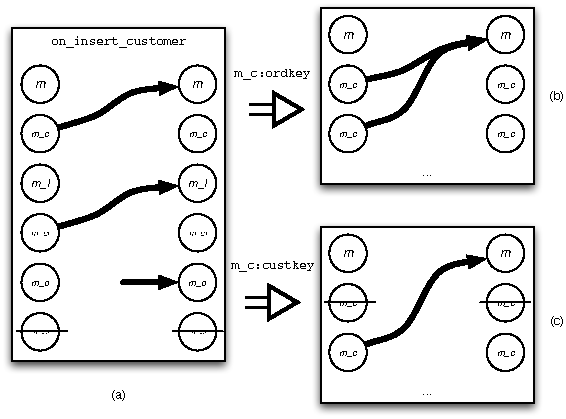
\includegraphics[width=2.5in]{graphics/MessagingGraph}
\end{center}
\caption{An example of a messaging graph based on Section \ref{sec:dbtoaster}'s example query.  (a) The messaging graph for the \texttt{on\_insert\_customer} event.  (b) The effects of splitting view $m_c$ on \texttt{ordkey}.  (c) The effects of splitting $m_c$ on \texttt{custkey}.}
\label{fig:diag:messagingGraph}
\vspace*{-0.2in}
\end{figure}

For example, consider the transition function that results from an update to the customer table.  One specific subtask of this transition reads $m_c$ and writes to $m$.  Treating each view as a node, this task has one edge with one read node and one write node.  

DBToaster considers database layout in terms of how it partitions data across a physical medium (i.e., memory, disk pages, or a cluster).  Viewed through the messaging graph, a partitioning is an assignment of all nodes in the graph to one (or more, in the case of replication) partition.  For example, if they were small enough, $m$ and $m_c$ might be placed on one disk page each.  Thus, the subtask requires a read on one page, and an update to a second.

Subdivision of individual views is represented in the messaging graph by splitting of graph nodes.  Of particular interest is how the new nodes interact with the hyperedge(s) connected to the original node.  As the split occurs, a node may stay connected to a hyperedge, the hyperedge may likewise be split, or in some cases, only one node will remain connected (see Figure \ref{fig:diag:messagingGraph}b,c).  DBToaster can exploit the limited range of node split/hyperedge interactions to select an effective partitioning scheme.

For example, when partitioning $m_c$, horizontal partitioning on the value of \texttt{ordkey} increases the number of nodes connected to the \texttt{on\_insert\_customer} task edge, while using \texttt{custkey} does not provoke an increase.  If the data represented by these nodes is split across multiple disks or servers, the computation must still access all of them.  The roles are reversed for the \texttt{on\_insert\_order} task edge.  Under (the false) assumption that both insert events occur with identical frequency, DBToaster can partition on both keys to minimize the number of connected nodes.

Additional knowledge about the dataset enhances the messaging graph produced by DBToaster.  For instance, the E-R diagram can be integrated into the messaging graph; the chain of foreign key dependencies in $q$ is strictly hierarchical.  DBToaster uses this information and creates partitions along a single axis with a secondary index to bound the number of partitions accessed by each update subtask, with respect to the total number of partitions generated.  Similarly, this information is used by DBToaster to select a partitioning scheme that places nodes typically connected by a subtask into a single partition; this is analagous to co-clustering in a traditional DBMS.
